\documentclass[11pt]{article}

\usepackage[a4paper,margin=1in]{geometry}
\usepackage{amsmath,amssymb}
\usepackage{booktabs}
\usepackage{graphicx}
\usepackage[colorlinks=true,linkcolor=blue,citecolor=blue,urlcolor=blue]{hyperref}
\newcommand{\SI}[2]{#1\,#2}
\newcommand{\vW}{\mathbf{W}}

\title{AVC, parameters adaption analysis and comparisons}
\author{Marco Falotico}
\date{\today}

\begin{document}
\maketitle

% \begin{abstract}
% The AVC algorithm of Muradore et al.\ adapts four state variables---the
% plant response $(x_1,x_2)$ and the disturbance quadratures
% $(x_3,x_4)$---plus the frequency and phase $(\omega,\alpha)$ of an
% auxiliary phase-locked loop. We show that these three groups have entirely
% different observability status: the frequency is observable, the
% disturbance quadratures are observable \emph{provided the plant is held
% fixed}, and the plant itself is never observable from a single tone. The
% algorithm should therefore adapt $(\omega,\alpha)$ and $(x_3,x_4)$ only,
% and take the plant from calibration. A five-configuration ablation in a
% closed-loop AO simulation confirms this exactly: removing frequency
% adaptation destroys cancellation ($+0.2$\,dB), adding plant adaptation
% destroys it as well ($+0.0$\,dB), and the recommended pair achieves
% $-37.4$\,dB.
% \end{abstract}

\section{What the measurement contains}

Write the plant response, the disturbance and the control as complex
numbers, $P=x_1+ix_2$, $\Lambda=x_3+ix_4$,
$\vartheta=\theta_c+i\theta_s$. The algorithm's control law (its eq.~11)
is then simply $\vartheta=-\hat\Lambda/\overline{\hat P}$: the estimated
disturbance divided by the estimated plant.

The algorithm models the measured residual as a sinusoid at the tracked
frequency,
\begin{equation}
  y(t)=\mathrm{Re}(Z)\cos\alpha(t)+\mathrm{Im}(Z)\sin\alpha(t),
  \qquad
  Z \;=\; \vartheta\,\overline{P_\star}+\Lambda_\star
    \;=\; \Lambda_\star-\kappa\,\hat\Lambda,
  \qquad
  \kappa=\overline{\left(\frac{P_\star}{\hat P}\right)},
  \label{eq:Z}
\end{equation}
where $P_\star,\Lambda_\star$ are the true plant and disturbance.

Once the phase $\alpha(t)$ is known, the measurement therefore depends on
the unknown parameters \emph{only} through the complex number $Z$ --- two
real numbers. This is not a sampling-rate statement: a \SI{47}{Hz} tone
sampled at \SI{1}{kHz} gives $\sim\!21$ points per period, but they are 21
noisy views of the same two numbers. Nor does it improve with time: since
the regressor is
$\vW=\cos\alpha\,\mathbf{u}_1+\sin\alpha\,\mathbf{u}_2$ with
$\mathbf{u}_{1,2}$ phase-independent, $\sum_t\vW\vW^\top$ has rank two for
any number of samples (verified over several hundred periods). More data
buys precision on those two numbers, never additional rank. So the whole
experiment yields two real numbers about the static parameters, and the
question of which parameters to adapt is the question of which of them are
determined by $Z$.

\section{Three groups, three different answers}

\subsection*{(a) The plant $(x_1,x_2)$: never observable}

Treating $(P,\Lambda)$ as jointly unknown, the map $(P,\Lambda)\mapsto Z$
is from $\mathbb{R}^4$ to $\mathbb{R}^2$ and has a two-dimensional kernel,
\begin{equation}
  \delta Z=\vartheta\,\overline{\delta P}+\delta\Lambda=0
  \quad\Longleftrightarrow\quad
  \delta\Lambda=-\vartheta\,\overline{\delta P}.
  \label{eq:kernel}
\end{equation}
Any change in the plant estimate can be exactly absorbed by a change in the
disturbance estimate, leaving every measurement unchanged at every phase,
for all time. The ambiguity is physical, not numerical: an experiment whose
entire yield is one complex number cannot determine two complex unknowns,
however long it is run. It cannot be
removed by descending the cost more accurately, nor by enriching the
disturbance; it would require an independent, known excitation of the
command, which is precisely what an offline probe measurement does.

The plant is not merely hard to estimate---it is \emph{not needed} as an
estimate. By \eqref{eq:Z} only $\kappa$ enters, and only through the sign
of the feedback: the loop of Sec.~(b) converges iff $\mathrm{Re}\,\kappa>0$,
i.e.
\begin{equation}
  \big|\arg P_\star-\arg\hat P\big|<90^\circ .
  \label{eq:margin}
\end{equation}
A magnitude error in $\hat P$ does not degrade the steady state at all: it
only rescales the converged $\hat\Lambda$. What the algorithm needs from
the plant is a phase, to within a very generous margin --- a calibration
constant, not a state.

\subsection*{(b) The disturbance quadratures $(x_3,x_4)$: observable once the plant is fixed}

Hold $\hat P$ fixed. Then \eqref{eq:Z} is an affine bijection between
$\hat\Lambda$ and $Z$ (slope $-\kappa\neq0$): two unknowns, two
measurements, exactly determined. Restricting the adaptation to
$(x_3,x_4)$ is therefore not a workaround for the degeneracy of
\eqref{eq:kernel} --- it is exactly the well-posed sub-problem that remains
once the unobservable directions are excluded.

The update that the algorithm performs on these components is,
after averaging over a cycle,
\begin{equation}
  \dot{\hat\Lambda}\;\propto\;Z\;=\;\Lambda_\star-\kappa\hat\Lambda,
\end{equation}
a first-order integral loop whose fixed point
$\hat\Lambda_\infty=\Lambda_\star/\kappa$ gives $Z=0$: \emph{exact}
cancellation of the tone, for any admissible $\hat P$. Note that
$\hat\Lambda$ converges to whatever command cancels the disturbance, not to
the disturbance itself; it is a controller state rather than an estimate.
(Measured over three runs with different $\hat P$, the converged
$|\hat\Lambda|$ tracks $|\hat P|$ to $\sim\!1\%$, as
$\hat\Lambda_\infty=\Lambda_\star/\kappa$ requires, while all three cancel
equally well.)

\subsection*{(c) The frequency $(\omega,\alpha)$: observable, and necessary}

A frequency error does not change the \emph{value} of $Z$ within a cycle;
it makes $Z$ \emph{rotate} from cycle to cycle, at rate
$\omega_\star-\hat\omega$. That rotation lies in the observable projection,
not in the kernel \eqref{eq:kernel}, and it is what the phase detector
$\langle y\sin\alpha\rangle$ of the PLL senses. Frequency is a property of
the observed signal itself, recoverable from the output alone; the plant,
by contrast, is a property of an input--output map that is never
independently excited.

Adaptation of $\omega$ is also \emph{necessary}. The pair $(x_3,x_4)$
integrating in the frame rotating at $\alpha$ is a resonant (internal
model) controller: its infinite loop gain sits exactly at $\hat\omega$ and
nowhere else. If $\hat\omega\neq\omega_\star$, the integrand rotates and
averages towards zero, and the correction collapses.

\subsection*{Summary}

\begin{center}
\begin{tabular}{lll}
  \toprule
  parameters & status & treatment\\
  \midrule
  $\omega,\alpha$ & observable (rotation of $Z$), and required & \textbf{adapt} (PLL)\\
  $x_3,x_4$       & observable once $\hat P$ is fixed; exactly determined & \textbf{adapt} (integral)\\
  $x_1,x_2$       & in the kernel; only $\arg\hat P$ matters, to $90^\circ$ & \textbf{calibrate, freeze}\\
  \bottomrule
\end{tabular}
\end{center}

\section{Experimental test}

Closed-loop single-conjugate AO simulation (\SI{64}{px} pupil, $8\times8$
Shack--Hartmann, 40 modes, \SI{1}{kHz}, integrator gain $0.5$ with 2-frame
delay, \SI{80}{Hz} actuator low-pass), with a \SI{120}{nm} tip vibration at
\SI{47}{Hz} that the loop \emph{amplifies} to a \SI{890}{nm} residual. AVC
acts on mode~0 in parallel with the integrator. Five \SI{5}{s} runs share
the atmospheric seed and vibration realisation and differ only in which
parameters are adapted; the plant seed, where used, is the measured
closed-loop value. Statistics over the second half of each run.

\begin{table}[h]
  \centering\small
  \begin{tabular}{lrrrrr}
    \toprule
    adapted parameters & mode-0 RMS & \SI{47}{Hz} amp. & vs.\ base & PSD vs.\ input & final $\hat f$\\
    \midrule
    none (no AVC)                                   & \SI{629.8}{nm} & \SI{890.3}{nm} & ---        & $+17.4$\,dB & ---\\
    $x_3,x_4$ only, $\omega$ fixed \emph{wrong} (45\,Hz) & \SI{646.2}{nm} & \SI{913.6}{nm} & $+0.2$\,dB & $+17.6$\,dB & 45.00\\
    $\omega,\alpha+x_3,x_4+x_1,x_2$ (original)      & \SI{634.8}{nm} & \SI{892.6}{nm} & $+0.0$\,dB & $+17.4$\,dB & 46.95\\
    $x_3,x_4$ only, $\omega$ fixed \emph{true} (47\,Hz)  & \SI{20.7}{nm}  & \SI{16.7}{nm}  & $-34.5$\,dB & $-16.1$\,dB & 47.00\\
    $\boldsymbol{\omega,\alpha+x_3,x_4}$ \textbf{[recommended]} & \textbf{\SI{26.1}{nm}} & \textbf{\SI{12.1}{nm}} & $\mathbf{-37.4}$\,\textbf{dB} & $\mathbf{-18.2}$\,\textbf{dB} & 47.00\\
    \bottomrule
  \end{tabular}
  \caption{Ablation over the adapted parameter set. Both departures from
  the recommended set --- removing frequency adaptation, or adding plant
  adaptation --- destroy cancellation completely. The last-but-one column
  gives the residual PSD at \SI{47}{Hz} relative to that of the injected
  disturbance (Fig.~\ref{fig:psd}): the uncontrolled loop \emph{amplifies}
  the tone by $17.4$\,dB, the recommended set puts it $18.2$\,dB below the
  input.}
  \label{tab:abl}
\end{table}

\begin{figure}[htbp]
  \centering
  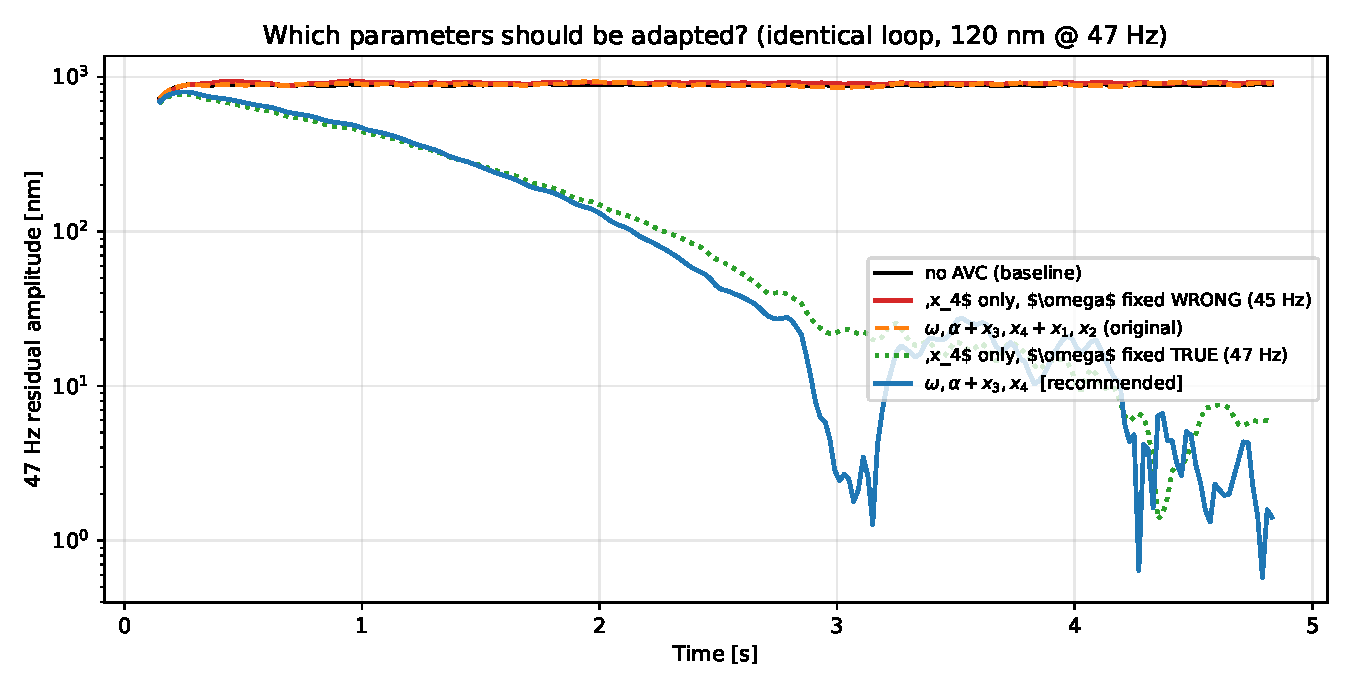
\includegraphics[width=0.92\textwidth]{avc_observability_ablation.pdf}
  \caption{\SI{47}{Hz} residual amplitude (\SI{300}{ms} lock-in). The two
  failing configurations sit on the baseline; the two working ones fall by
  more than a decade.}
  \label{fig:abl}
\end{figure}

\begin{figure}[htbp]
  \centering
  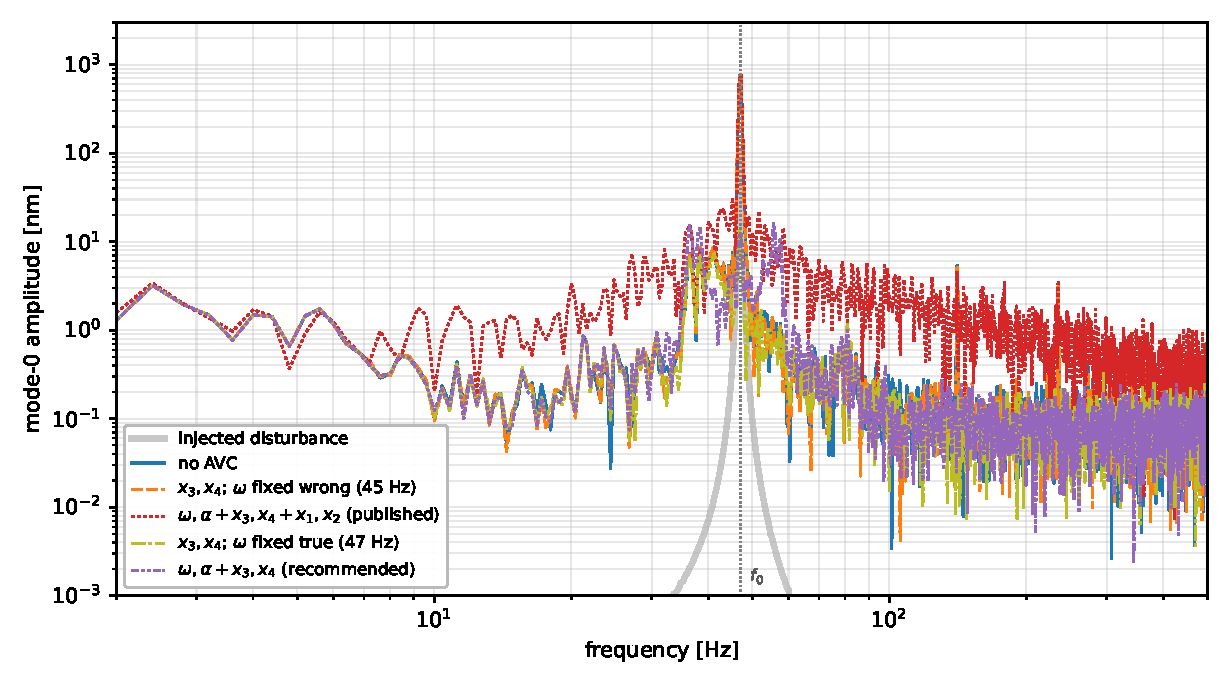
\includegraphics[width=0.98\textwidth]{avc_ablation_psd.pdf}
  \caption{Steady-state mode-0 residual PSD for each configuration,
  together with the PSD of the injected disturbance (grey). The loop
  \emph{amplifies} the tone: without AVC the residual peak stands
  $+17.4$\,dB \emph{above} the input. The two failing configurations track
  the baseline peak exactly; the two working ones remove it entirely,
  leaving the residual $-18.2$\,dB \emph{below} the input --- a
  \SI{35.6}{dB} swing at the tone. Note also the raised broadband floor of
  the original update (orange), $\sim\!1$--$2$ decades above every other
  configuration across the whole band: an unusable, wrongly-phased
  correction is being injected at all frequencies.}
  \label{fig:psd}
\end{figure}

The table matches the analysis line by line.
\begin{itemize}\itemsep2pt
  \item \textbf{Adapting $x_1,x_2$ destroys cancellation} ($+0.0$\,dB),
    even though this run starts from the exactly measured plant. The
    unobservable directions \eqref{eq:kernel} are free to drift, $\arg\hat P$
    wanders, the margin \eqref{eq:margin} is violated and the integral loop
    of Sec.~(b) reverses sign.
  \item \textbf{Not adapting $\omega$ destroys cancellation too}
    ($+0.2$\,dB) when the frequency is held \SI{2}{Hz} away from the truth
    --- a large error for a resonant controller whose gain is concentrated
    at $\hat\omega$.
  \item \textbf{Holding $\omega$ at the true value works} ($-34.5$\,dB),
    confirming that the PLL's only job is to find $\omega$; and the PLL
    started \SI{2}{Hz} away recovers that performance and slightly exceeds
    it ($-37.4$\,dB), having converged to \SI{47.00}{Hz}.
  \item \textbf{The spectra separate the two failure modes}
    (Fig.~\ref{fig:psd}). Fixing $\omega$ at the wrong value leaves the
    residual spectrum indistinguishable from the baseline: the resonant
    controller is simply tuned elsewhere and does nothing. Adapting
    $x_1,x_2$, by contrast, leaves the \SI{47}{Hz} peak untouched
    \emph{and} lifts the broadband floor by one to two decades across the
    whole band --- the wandering plant estimate produces a large,
    wrongly-phased command that injects noise everywhere without cancelling
    anything. The second failure is therefore strictly worse than doing
    nothing.
\end{itemize}

\section{Conclusion}

The three parameter groups of the AVC algorithm are not interchangeable.
The frequency is observable from the time evolution of the measured phasor
and must be adapted, because the correction is a resonant controller tuned
to it. The disturbance quadratures are exactly determined once the plant is
held fixed, and their update is the integral action that performs the
cancellation. The plant lies entirely in the unobservable kernel: it cannot
be identified from a single tone, it is not needed beyond a phase accurate
to $90^\circ$, and adapting it online is not merely futile but actively
destabilising. Adapt $(\omega,\alpha)$ and $(x_3,x_4)$; calibrate the
plant and leave it alone.

\paragraph{Reproducibility.}
Runs generated from \texttt{params\_scao\_avc\_full\_demo.yml} with the
\texttt{gomega}, \texttt{freq} and \texttt{adapt\_plant} keys of the
\texttt{avc:} block set as tabulated, against
\texttt{params\_scao\_vibration\_baseline.yml}. Companion reports:
\texttt{avc\_hybrid\_note.pdf} (exact differentiation and why the cost is
not a control objective) and \texttt{avc\_exact\_gradient.pdf} (full
analysis).

\end{document}
